\documentclass[10pt,twocolumn,letterpaper]{article}
\usepackage[margin=0.75in,columnsep=0.25in]{geometry}
\usepackage{amsmath,amssymb,booktabs,array,graphicx}
\usepackage{tikz,pgfplots}
\pgfplotsset{compat=1.18}
\usepackage{xurl}
\usepackage[hidelinks]{hyperref}
\urlstyle{same}
\setlength{\emergencystretch}{1em}
\setlength{\parskip}{0pt}
\raggedbottom
\setlength{\textfloatsep}{10pt plus 2pt minus 2pt}
\setlength{\floatsep}{9pt plus 2pt minus 2pt}
\newcommand{\bx}{\textsc{Bitoxin}}
\newcommand{\code}[1]{\texttt{#1}}
\title{BITOXIN: Preserving State Dependencies to Expose\\Integrity Failures in Stateful Testing}
\author{Anonymous Author(s)}
\date{October 5, 2026}
\hypersetup{pdftitle={BITOXIN: Preserving State Dependencies to Expose Integrity Failures in Stateful Testing},pdfauthor={Anonymous Author(s)},pdfsubject={Test-design method and controlled observability experiments}}
\begin{document}
\maketitle

\begin{abstract}
State corruption may escape detection during testing when tests discard live state before checking it, reuse an unchecked result as their expectation, or observe only values that no longer depend on the corrupted state. This paper presents BITOXIN as a test-design method that combines persistent state, dependent operations, permitted execution interruptions, and independently specified observations. The method draws on established stateful-testing and fault-observability ideas; its reference implementation is a resumable integrity probe, not a prerequisite for product adoption. We specify its detection assumptions and evaluate observation policies through 61,440 enumerated single-bit-injection trials and 120 clean controls. For faults inserted at five bit-walk boundaries, retaining state and performing a final scan detects all 15,360 faults assigned to that policy. Omitting the scan detects 7,680; reconstructing clean state detects none. A further 15,360 trials show that corruption behind an advancing verifier can escape the current pass but is detected in the next retained pass under the stated model. Native ARM64, portable-C, and sanitizer configurations produce identical outcome records. These results validate a narrow observation mechanism rather than establish field defect coverage or improved time to discovery. We also describe how to transfer the method to protected-value libraries and transaction services without deploying a Linux module.
\end{abstract}
\par\smallskip
\noindent\textbf{Keywords:} stateful testing; fault observability; integrity checking; fault injection; system testing

\section{Introduction}
A system can execute a large workload without exposing every incorrect intermediate state to a test oracle. An overwritten value, an early reinitialization, or an unchecked cache may separate a fault from an observable failure. This distinction matters in systems whose behavior spans scheduling, memory ownership, session lifetimes, and device transitions. Production reports on silent data corruption show why computational errors and their eventual application-level manifestations must be considered together~\cite{dixit2022}.

The practical question addressed here is: \emph{how should a test workload preserve and observe the state whose integrity it intends to test?} Merely increasing work does not answer that question. Nor does a long sequence imply that every intermediate error affects its final result. For example, multiplication by zero can erase an earlier arithmetic error, while rebuilding an object after a transition can destroy evidence of corruption that occurred during the transition.

\bx\ originated in an embedded-system testing workflow that ran an independent computation alongside system activity, including sleep/wakeup cycles. Its motivating hypothesis has two parts: background activity may bring a system into conditions that activate a latent defect, while a dependent computation retains and exposes resulting corruption. The computation must remain interruptible so that the activities can interact with its live state. The practical aim was to make a silent error recognizable to an external test executor, historically through a crash; an explicit mismatch report can serve that purpose without a crash. Historical field recollections are not experimental evidence here. We reconstruct the method and evaluate its observation mechanism under a finite fault model; increased activation and faster discovery of natural defects remain untested hypotheses.

The reusable concept is independent of execution layer. A protected-value library can carry actual objects through arithmetic and lifecycle operations; a transaction service can retain request, buffer, and response history. Neither application requires running the reference Linux module beside the product. The product's own state and its contract become the test subject.

This paper makes three bounded contributions:
\begin{enumerate}
\item A design contract connecting state lifetime, data dependency, allowed interruptions, and independent observations, including conditions that invalidate an inference of detection.
\item A resumable reference probe with explicit traversal and verification invariants, supported by algorithmic, host, and virtual-kernel checks.
\item Reproducible, enumerated fault experiments that separate retaining state, checking visited locations, and extending the observation horizon.
\end{enumerate}
The contribution is an engineering method and its executable analysis. We do not claim to originate stateful testing, error propagation, or test oracles; establish a new universal coverage metric; or demonstrate superiority to existing testing tools.

\section{Background and Positioning}
\paragraph{Fault observation.}
The reachability, infection, propagation, and revealability (RIPR) model separates executing a faulty location from observing its consequences~\cite{ammann2017}. BITOXIN adopts that distinction as a design discipline: exercise relevant conditions, retain affected state, and specify an observation that can distinguish an error. A dependent instruction sequence alone does not satisfy all of these requirements.

\paragraph{Stateful and model-based testing.}
Wei et al. generate tests using inferred contracts to seek states not adequately exercised by an existing suite~\cite{wei2011}. Hypothesis supports action sequences, reuse of values produced by earlier rules, comparison with a reference model, and invariants checked between steps~\cite{hypothesis}. These capabilities can host the product-level method described here. BITOXIN's emphasis is the integrity of live state across interruptions and the explicit validation of its observation horizon, rather than a new sequence-generation algorithm.

\paragraph{Metamorphic relations.}
Metamorphic testing uses relations among multiple executions when direct expected outputs are difficult to obtain~\cite{chen2018}. Identity and round-trip computations can supply useful relations, but related executions may share faults. Our reference probe uses an identity register transformation with a direct input/output comparison and separate memory expectations. Product adaptations should combine applicable relations with known answers or independent models.

\paragraph{Scheduling and event order.}
CHESS systematically explores thread interleavings and supports reproduction of failures~\cite{chess2008}. Event-sequence covering methods exercise specified orders among events~\cite{kuhn2012}. Both are complementary to the observation structure considered here. BITOXIN permits scheduling and records test progress; it neither controls all schedules nor claims exhaustive event-order coverage. A seed identifying a memory traversal is not a replay of execution timing.

\paragraph{Stress and computational integrity.}
Stressful Application Test generates memory and I/O traffic and checks data integrity~\cite{stressapptest}. Dixit et al. discuss in-production and out-of-production strategies for detecting silent corruption at scale~\cite{dixit2022}. These are relevant operational contexts, but our experiments do not compare their detection performance. We isolate a smaller question: what happens to a known injected error when a test retains, checks, or reconstructs the state containing it?

\section{A Design Contract for Stateful Testing}
\subsection{State, events, and observations}
Let $x_i$ be the actual product state before step $i$, $u_i$ its intended operation input, and $e_i$ an event permitted by the product contract. A useful abstraction is
\begin{equation}
 x_{i+1}=F_i(E_{e_i}(x_i),u_i),\qquad
 r_{i+1}=G_i(r_i,u_i,e_i),
\end{equation}
where $r_i$ is a separately maintained reference state. $E$ represents an interruption or transition; $G$ encodes its specified effect, including invalidation or rejection when applicable. An observation predicate $V_i(O_i(x_i),r_i)$ is evaluated at selected checkpoints. The oracle should not silently adopt an unchecked actual output as its new reference.

Figure~\ref{fig:contract} illustrates the two paths. The actual path retains product outputs as inputs to later operations. The reference path follows intended inputs and specified event semantics. Checkpoints connect the paths without repairing the product from the reference. A reference may be simpler than the product, but merely calling the same faulty routine twice does not make it independent.

\begin{figure}[t]
\centering
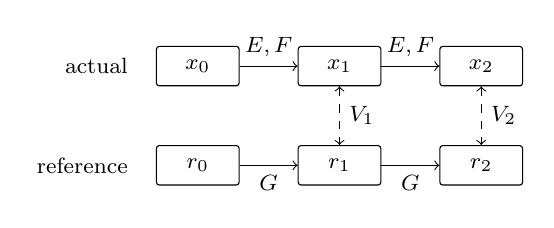
\begin{tikzpicture}[x=0.9cm,y=0.9cm,every node/.style={font=\footnotesize},box/.style={draw,rounded corners=1pt,minimum width=1.05cm,minimum height=.50cm}]
\node[box] (x0) at (0,1.4) {$x_0$};
\node[box] (x1) at (2,1.4) {$x_1$};
\node[box] (x2) at (4,1.4) {$x_2$};
\node[box] (r0) at (0,0) {$r_0$};
\node[box] (r1) at (2,0) {$r_1$};
\node[box] (r2) at (4,0) {$r_2$};
\draw[->] (x0) -- node[above] {$E,F$} (x1);
\draw[->] (x1) -- node[above] {$E,F$} (x2);
\draw[->] (r0) -- node[below] {$G$} (r1);
\draw[->] (r1) -- node[below] {$G$} (r2);
\draw[dashed,<->] (x1) -- node[right] {$V_1$} (r1);
\draw[dashed,<->] (x2) -- node[right] {$V_2$} (r2);
\node[anchor=east] at (-.85,1.4) {actual};
\node[anchor=east] at (-.85,0) {reference};
\end{tikzpicture}
\caption{Actual state survives between operations. A separate reference follows intended semantics; observations compare the paths without resetting actual state.}
\label{fig:contract}
\end{figure}

\subsection{Four requirements}
\paragraph{Retain the relevant history.}
Define when a value, handle, buffer, or session is created and retired. A fault can affect an observation only if its consequences survive until that observation. Resetting between independent tests is useful for isolation; resetting inside the interval whose integrity is being tested can erase the relevant history. Both forms of testing are needed for different questions.

\paragraph{Carry actual dependencies.}
The next product operation must consume the actual preceding state. A loop that performs many unrelated computations does not create that dependency. Check for masking operations, including truncation, overwrite, zeroing, and inverse transformations that can cancel correlated errors. Longer chains need not improve detection monotonically.

\paragraph{Permit meaningful interruptions.}
Do not serialize an entire test behind a lock if its purpose is to examine allowed interleavings. Conversely, introducing a data race forbidden by the API does not establish a product defect. Use documented synchronization and lifecycle rules. A transition may legitimately invalidate state; in that case, expected rejection is an observation, not a failure of the test design.

\paragraph{Specify what exposes the error.}
Check values, identities, lengths, generations, and required rejection outcomes as appropriate. Preserve the first mismatch and enough prefix history to reproduce it. Intermediate checkpoints can prevent later masking; an external observer is needed for hangs or resets that stop the checker itself. An assertion or typed failure is sufficient. Deliberately crashing the system is not essential to the concept.

\subsection{Probability and scope}
For a specified fault and a sound observation predicate, define a true detection as the conjunction of reachability $R$, infection $I$, propagation $P$, and revelation $O$. Then
\begin{align}
\Pr(\mathrm{detected})={}&\Pr(R)\Pr(I\mid R)\Pr(P\mid R,I)\nonumber\\
 &\cdot\Pr(O\mid R,I,P).
\end{align}
This identity, when the conditionals are defined, requires no independence assumption. Data dependency does not make successive failures statistically independent. Nor does a weighted average of state-dependent success probabilities bound every individual state from below. We use this decomposition to delimit claims, not to estimate an unknown system's reliability.

\paragraph{Coupling activation and observation.}
The method has separate activation and observation questions, although both activities share the system under test. A background scenario varies relevant load, lifecycle events, and configuration; the dependent computation carries live state across those events and checks for damage. The scenario need not directly control a power sequence. However, a workload may suppress an idle or gating condition that triggers a defect, so increased activity is not automatically useful coverage. Software injection evaluates whether a specified corruption remains observable; it does not show that either activity activates natural faults more often. A complete system-testing campaign therefore needs evidence of reached conditions as well as recorded failures. A supervisor should distinguish a reported mismatch from a hang or restart and retain run identity and progress across recovery where possible. Such an interruption alone does not identify corruption as its cause.

\section{Reference Integrity Probe}
\subsection{Traversal and invariants}
The reference engine maintains a private buffer of $B$ bytes with $N=8B=2^m$ bits, an expected bit polarity, and traversal and verification cursors. Supported engine sizes range from 64 bytes to 128 MiB. A right-shift Galois LFSR visits the $N-1$ nonzero bit indices; bit zero is visited explicitly. LFSRs provide compact deterministic sequences~\cite{alfke1996}; maximality is checked for the actual masks and convention used by this implementation.

Initially every byte is \code{0xff}. During a bit visit, the engine reads the containing byte, checks the selected bit against its expected polarity, carries a token containing that byte through a register transformation, checks the transformed token, and stores the byte with the selected bit inverted. After exactly $N$ visits, it scans all $B$ bytes for the expected uniform endpoint. Only then does it increment the completed-pass count and invert the expected polarity. The same buffer continues into the next pass.

In a fault-free execution, a pass visits each bit exactly once and the final scan confirms either all zeros or all ones. A pass costs $N+B=9B$ logical probe operations, excluding initialization and control. The scan adds $B$ operations to an $8B$-operation walk, or 12.5\% by this accounting; this is not a measured runtime overhead. Two passes restore the initial bytes. A step budget limits work before returning control, without reinitializing state or making the steps atomic with respect to the scheduler.

\subsection{Register and execution contracts}
On ARM64, the token passes through a sequence of complement, rotate, and move instructions whose correct composite result is the input. The low byte is derived from the actual memory load and supplies the eventual store. Explicit input/output constraints, early-clobber output, and scratch-register clobbers express the compiler contract~\cite{gcc}. The implementation uses general-purpose registers and avoids reserved platform registers and floating-point state. Portable C provides a semantic reference, not equivalent physical register coverage.

The engine reports the first observed data, register-result, state, or configuration error. These labels identify checks, not root causes. A register-result mismatch does not independently identify a defective physical register. Subsequent calls preserve the latched failure.

The shared engine has a user-process runner and a Linux worker wrapper. Neither disables preemption around the computation. The kernel wrapper can cooperate with the task freezer while retaining its buffer and cursors~\cite{linuxfreezer}. A CPU executes no probe instructions while powered off; resumed execution inspects retained or restored state. PM notifications do not prove that a hardware sleep state was reached. These wrappers demonstrate one execution context for the method; product adoption can operate entirely in the product's existing test framework.

\subsection{Checker defects found during reconstruction}
Verification exposed a legacy degree-14 mask, \code{0x201d}, with period 126 under the implemented recurrence rather than the required 16,383. The replacement \code{0x3802} passes an independent linear-map order test. All 22 supported degrees, 9 through 30, satisfy the tested full-order conditions. This finding concerns a defect in the checker and must not be counted as a newly detected hardware defect.

A separate legacy hook loop performed one excess visit. The historically used independent-worker path did not have that loop boundary. The reconstructed engine uses explicit visit counts and closure checks. These examples motivate testing the checker before attributing its reports to the environment.

\section{Evaluation Design}
\subsection{Objectives and fault model}
The evaluation examines how state retention and a final scan affect observation of an injected bit flip, and what remains unobserved when corruption occurs behind a moving verification cursor. Separate implementation checks assess traversal correctness, register transformations, and execution behavior.

The new experiments enumerate a finite software fault model. Each trial begins from a correct prefix of the real C engine with $B=64$, $N=512$, one of seeds $\{1,17,255\}$, and one of the two pass directions. Exactly one buffer bit is XOR-flipped at a call boundary. The error persists unless the tested policy overwrites it. The harness, control state, oracle, and later operations are assumed correct. Calls have a budget of one logical probe operation; no concurrent fault is injected inside a load, store, or assembly sequence.

The seeds shift the same LFSR cycle and are not independent random permutations. Enumerating them checks phase consistency, not statistical independence. We count detections, clean-control failures, and attempted post-injection calls. A call that detects a mismatch counts as one attempt. Attempt counts are operation-scale latency, not elapsed time.

The protocol and analytical expectations were written before running these experiments. Production sources were not modified for injection. The harness is linked against the shared engine and changes only its own test buffer at declared boundaries.

\subsection{Experiment 1: retaining and observing state}
Inject after $k\in\{0,128,256,384,512\}$ completed bit visits and enumerate every target bit. Three policies operate on separate trials:
\begin{description}
\item[Retain + scan:] Continue with the corrupted state through the current pass's final scan.
\item[Walk only:] Retain the state but stop when the walk ends, before the scan.
\item[Reset + replay:] Reinitialize the state, reconstruct the clean prefix at the same boundary, and then finish the pass with a scan.
\end{description}
The last policy intentionally models loss of evidence through reconstruction; it is not a competitive testing tool. Its reconstruction cost is excluded from post-boundary attempt counts, and no performance comparison is made. Each policy has $5\times512\times3\times2=15{,}360$ injected trials and 30 clean controls.

Under this model, an unvisited corrupted bit fails its selected-bit check. A visited corrupted bit is preserved by subsequent correct updates to other bits and fails the final byte scan. Thus the predicted count per 512-bit group is 512 for Retain + scan, $512-k$ for Walk only, and zero for Reset + replay. This argument assumes a single persistent fault between operations; it does not cover arbitrary concurrent corruption or damage to the checker.

\subsection{Experiment 2: verification horizon}
Complete the walk, verify $q\in\{0,16,32,48,63\}$ bytes, and inject into every bit. Continue until detection or the next pass boundary, recording separately whether the current pass detected the error. There are another 15,360 injections and 30 clean controls.

A fault in an already verified byte can escape the current scan. The predicted current-pass detection count is $512-8q$ per 512-bit group. If execution retains the state into the following pass, the selected-bit check eventually reaches the corrupted bit. Under the stated model, all 512 locations are therefore detected by that following boundary. This experiment makes the observation horizon explicit instead of interpreting one completed scan as perpetual integrity.

\subsection{Environment and reproducibility}
The new campaign ran on macOS ARM64 with Apple Clang 21.0.0, using optimized native ARM64 and forced portable-C builds, and a native AddressSanitizer/UndefinedBehaviorSanitizer build. All three produced identical raw outcome rows. These are three executions of the same finite cases, not three independent populations of defects. Sanitizers do not instrument the assembly internals.

Separate preserved verification records cover Linux ARM64 with GCC 12.2.0, a warning-enabled module build against Linux 6.1.0-53 ARM64 headers, and a QEMU 7.2.22 guest with two Cortex-A53 virtual CPUs. The virtual-kernel PM check uses \code{pm\_test=freezer}; it does not execute physical sleep. Experiment scripts, compressed trial data, compiler records, and source hashes accompany the manuscript.

\section{Results}
\subsection{Retention and final scanning}
Table~\ref{tab:walk} reports detections at each injection boundary, pooled over seeds and directions. Retain + scan detected 15,360 of its 15,360 injected faults. Walk only detected 7,680 of 15,360, and Reset + replay detected zero of 15,360. All 90 clean controls completed without a report. Figure~\ref{fig:results} shows the exact finite-case fractions.

\begin{table}[t]
\centering\small
\caption{Experiment 1: detections out of 3,072 injections per cell. $k$ is the number of completed bit visits.}
\label{tab:walk}
\begin{tabular}{r r r r}
\toprule
$k$ & Retain + scan & Walk only & Reset + replay \\
\midrule
0 & 3,072 & 3,072 & 0 \\
128 & 3,072 & 2,304 & 0 \\
256 & 3,072 & 1,536 & 0 \\
384 & 3,072 & 768 & 0 \\
512 & 3,072 & 0 & 0 \\
\bottomrule
\end{tabular}

\end{table}

The 50\% aggregate for Walk only is a consequence of the chosen, equally weighted boundaries. It is not an estimated field detection probability. At the midpoint, the policy misses exactly the already visited half of the bits. The final scan provides an observation for those locations; reconstruction removes the error before either mechanism can observe it. These are mechanism checks against deliberately weakened policies, not evidence of superiority to mature memory-test tools.

\subsection{The observation horizon}
Table~\ref{tab:scan} shows that current-pass detection declines with the number of already verified bytes. At $q=63$, only 48 of 3,072 cases are detected before that pass completes; the other 3,024 cases involve bytes behind the cursor. All 15,360 scan-boundary faults are detected by the end of the following retained pass. The maximum observed post-injection detection latency across these cases is 560 attempted probe operations. All 30 additional clean controls complete without a report.

\begin{table}[t]
\centering\small
\caption{Experiment 2: detections out of 3,072 injections per row. The following-pass column includes earlier detections.}
\label{tab:scan}
\begin{tabular}{r r r r}
\toprule
$q$ & Current pass & By following pass & Max. attempts \\
\midrule
0 & 3,072 & 3,072 & 64 \\
16 & 2,304 & 3,072 & 560 \\
32 & 1,536 & 3,072 & 544 \\
48 & 768 & 3,072 & 528 \\
63 & 48 & 3,072 & 513 \\
\bottomrule
\end{tabular}

\end{table}

Across both experiments there are 61,440 injected trials and 120 clean controls per build configuration. Zero observed clean-control failures means only that these bounded controls did not falsely report a mismatch. The deterministic enumeration does not support inferential confidence intervals for hardware defect coverage.

\begin{figure}[t]
\centering
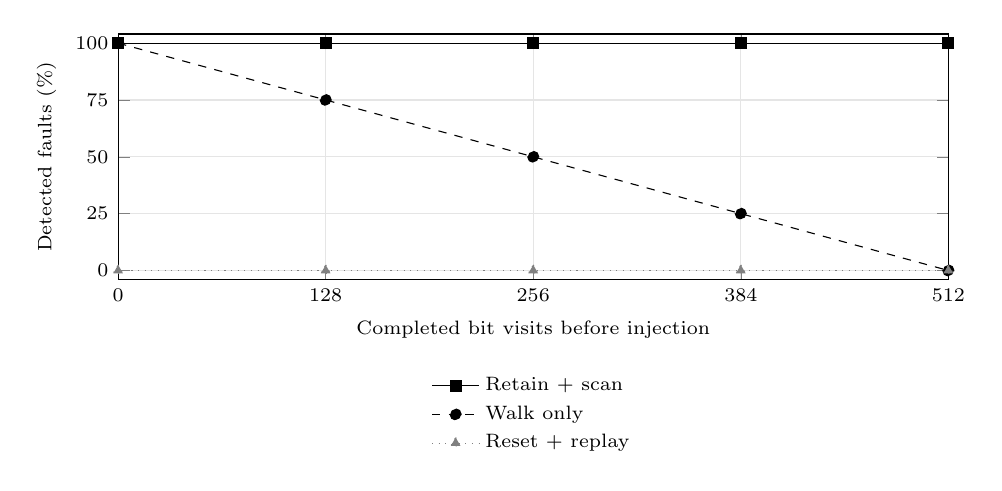
\begin{tikzpicture}
\begin{axis}[width=\columnwidth,height=4.7cm,
xlabel={Completed bit visits before injection},ylabel={Detected faults (\%)},
xmin=0,xmax=512,ymin=-4,ymax=104,xtick={0,128,256,384,512},ytick={0,25,50,75,100},
tick label style={font=\scriptsize},label style={font=\scriptsize},
legend style={font=\scriptsize,at={(0.5,-0.35)},anchor=north,draw=none},
grid=major,grid style={gray!20},legend cell align=left]
\addplot[black,mark=square*] coordinates {(0,100) (128,100) (256,100) (384,100) (512,100)};
\addlegendentry{Retain + scan}
\addplot[black,dashed,mark=*] coordinates {(0,100) (128,75) (256,50) (384,25) (512,0)};
\addlegendentry{Walk only}
\addplot[gray,dotted,mark=triangle*] coordinates {(0,0) (128,0) (256,0) (384,0) (512,0)};
\addlegendentry{Reset + replay}
\end{axis}
\end{tikzpicture}

\caption{Observed fractions for the enumerated model. Each point pools 3,072 injections. Lines connect discrete boundaries; they are not a fitted probability model.}
\label{fig:results}
\end{figure}

\subsection{Implementation checks}
The independent order tests cover all 22 LFSR masks. Register-lane checks compare 10,128 chosen input patterns with their expected identity outputs. Core tests cover full and inverse passes, bit zero, chunked continuation, early and late corruption, malformed cursors, invalid configuration, and latched errors. A test-only lane substitution confirms that an altered output is rejected before the corresponding buffer write. It is a simulated output error, not a physical register fault.

Native, portable, sanitizer, and Linux user-space tests pass in the recorded environments. The virtual-kernel run demonstrates bounded two-worker completion, retained cursors across freezer tests, unloading active workers, and five repeated load/unload cycles. Startup resource-failure injection and the actual panic path remain unexecuted. None of these checks establishes a physical interruption inside a particular assembly instruction, target-board qualification, or real power-sequence coverage.

\section{Product Applications}
The following are application designs, not evaluated integrations. The test adapter should expose product operations and observations, while an independent model represents values, ownership, and lifetimes. Sequence generation may be random, covering-based, or hand-authored. The essential requirement is that it operates on actual retained product state.

\subsection{Protected-value libraries}
Consider a library that represents values through protected storage and session-scoped handles. A test can create $x=37$, add 11, copy $x$ to $y$, permit an allowed scheduling boundary, multiply $y$ by 3, and subtract 5 from $x$. A separate arithmetic model expects $x=43$ and $y=144$. The test then continues with those objects rather than reconstructing them from expected values.

Checks should exercise the protected representation, not merely a cached plaintext result. Use bounded integer arithmetic to avoid undefined overflow in the test. Across key rotation or shutdown, model the documented preservation or invalidation contract: an invalid handle should yield the specified rejection, while a state promised to survive must continue to produce the expected result. Positive controls prevent a disabled implementation from passing by rejecting every operation.

Identity relations remain useful, but a chain consisting only of zero values or inverse pairs can hide errors. Intermediate checkpoints and controlled test faults assess whether corrupted state reaches the intended verification interface. This is a library-test design; no kernel integration is implied.

\subsection{Stateful transaction services}
For a service using framed requests and shared buffers, carry a transaction through begin, input transfer, execute, and read operations. Check request identity, status, output length, and an independently known result. Continue with a distinct subsequent request while retaining service and buffer history so stale data and ownership mistakes remain observable.

Vary permitted fragmentation, descriptor offsets, buffer reuse, and ownership handoffs. Negative sequences require explicit expected status and post-rejection state. A timeout, abort, or reconnect need not preserve a request transparently unless the protocol promises that behavior. Fault injection belongs at defined, test-owned interfaces.

For cryptographic computation, compare deterministic byte or coefficient fixtures exactly and approximate decoded values using the profile's specified scale and tolerance. Keep independent known answers rather than relying solely on a round trip that can share an implementation error. A host simulator validates these contracts; it does not establish physical shared-memory coherency or retention across power loss.

\subsection{A product-level comparative study}
A subsequent evaluation should cross two factors: independent short cases versus linked cases, and baseline conditions versus a defined background activity or transition scenario. This separates the effect of retaining dependencies from the background scenario and allows their interaction to be examined. Match operation mix, operation count, resource budgets, and observation duration where possible. Record reached conditions, including completed transitions rather than requests alone. Separate injected-fault detection from confirmed natural defects. Record first valid failure time, unique root causes, reproduction denominators, false reports, and test overhead; retain runs without an observed failure as censored observations where time-to-event analysis is used.

When minimizing a failure, preserve the prefix that establishes the relevant state and event order. Confirm attribution by fixing the product defect and rerunning the same scenario. This study has not yet been conducted for either application design.

\section{Threats to Validity}
\paragraph{Fault-model validity.}
Single persistent buffer-bit flips at call boundaries are a restricted model. Real failures may be transient, correlated, multi-bit, control-flow related, or capable of corrupting the checker and its reference simultaneously. We test neither physical fault activation nor adversarial resilience. The enumerated detections cannot be generalized to all faults, instructions, or devices.

\paragraph{Internal validity.}
The same harness drives the policies, so a harness bug could affect all results. To reduce that risk, group counts are checked against independently specified arithmetic expectations, reported error locations are checked against injection locations, and outcome rows are compared across native, portable, and sanitizer configurations. The policies share the engine; the experiment is an ablation of observation behavior, not an independent reimplementation or an external-tool benchmark.

\paragraph{External validity.}
The injection buffer has only 64 bytes. It does not exercise realistic cache capacities, paging behavior, DDR traffic, or heterogeneous memory. The LFSR's exhaustive bit-index traversal is not exhaustive coverage of system states or instruction $n$-grams. A cache hit need not access DRAM. The virtual-kernel tests cannot reproduce electrical effects of clock gating, voltage transitions, or memory retention.

\paragraph{Measurement and operational validity.}
We report logical attempts, not timing or throughput. Checking changes the workload and may alter the very condition being investigated. More activity can prevent low-power entry. An absence of reported corruption is not a reliability certificate, and structured logs can be lost in a crash or power failure. Independent workload and transition observations are needed in real system-testing campaigns.

\paragraph{Scope of the evidence.}
The experiments demonstrate specified observability properties and checker behavior. They do not show faster discovery of previously unknown product defects, validate the historical embedded-system anecdote, or measure the proposed product adaptations. Establishing those claims requires external comparative experiments.

\section{Conclusion}
BITOXIN expresses a practical testing requirement: preserve the state whose integrity matters, carry it through meaningful dependencies and allowed interruptions, and observe it against an independent expectation. Its original motivation couples background scenarios that may activate defects with a computation that exposes resulting corruption. The finite fault experiments validate the observation side: reinitialization, omitted endpoint checks, and an advancing verifier change what a test can reveal. They do not validate the activation side or faster defect discovery. The concept can be applied within product test frameworks without adopting the original kernel execution model. Its combined effect remains a question for controlled product and hardware campaigns.

\section*{Artifact Availability}
The ancillary supplement contains the measured core, controlled-injection harness, declared protocol, compressed per-trial data, build summaries, and file hashes. The new observability experiments can be reproduced independently with a C11 compiler and Python 3, without a kernel module. Earlier host and virtual-kernel verification records are supplied separately as evidence; those wrapper checks require the full repository. The manuscript source includes the tables and plot generated from the recorded data. The supplement distinguishes these measured checks from the proposed product applications.

\bibliographystyle{unsrt}
{\raggedright\bibliography{references}}
\end{document}
